\documentclass[10pt]{article}
\usepackage[letterpaper,text={6.5in,8.6in},centering]{geometry}
\usepackage{amssymb,amsmath,amsthm,times,graphicx,subfigure}
\usepackage{enumitem}
\usepackage{trimclip} % for AR symbol
\usepackage{nomencl} % nomenclature
\usepackage{siunitx}
\usepackage[paper=portrait,pagesize,DIV=13]{typearea}
\usepackage{array} % for math mode in table
\usepackage{multicol}
\usepackage{float}
\usepackage{hyperref}
\usepackage{cleveref}
\usepackage{tikz}
\usetikzlibrary{arrows}

\newcommand{\norm}[1]{\ensuremath{\left\| #1 \right\|}}
\newcommand{\bracket}[1]{\ensuremath{\left[ #1 \right]}}
\newcommand{\braces}[1]{\ensuremath{\left\{ #1 \right\}}}
\newcommand{\parenth}[1]{\ensuremath{\left( #1 \right)}}
\newcommand{\pair}[1]{\ensuremath{\langle #1 \rangle}}
\newcommand{\met}[1]{\ensuremath{\langle\langle #1 \rangle\rangle}}
\newcommand{\refeqn}[1]{(\ref{eqn:#1})}
\newcommand{\reffig}[1]{Fig. \ref{fig:#1}}
\newcommand{\tr}[1]{\mathrm{tr}\ensuremath{\negthickspace\bracket{#1}}}
\newcommand{\trs}[1]{\mathrm{tr}\ensuremath{[#1]}}
\newcommand{\ave}[1]{\mathrm{E}\ensuremath{[#1]}}
\newcommand{\deriv}[2]{\ensuremath{\frac{\partial #1}{\partial #2}}}
\newcommand{\SO}{\ensuremath{\mathsf{SO(3)}}}
\newcommand{\T}{\ensuremath{\mathsf{T}}}
\renewcommand{\L}{\ensuremath{\mathsf{L}}}
\newcommand{\so}{\ensuremath{\mathfrak{so}(3)}}
\newcommand{\SE}{\ensuremath{\mathsf{SE(3)}}}
\newcommand{\se}{\ensuremath{\mathfrak{se}(3)}}
\renewcommand{\Re}{\ensuremath{\mathbb{R}}}
\newcommand{\aSE}[2]{\ensuremath{\begin{bmatrix}#1&#2\\0&1\end{bmatrix}}}
\newcommand{\ase}[2]{\ensuremath{\begin{bmatrix}#1&#2\\0&0\end{bmatrix}}}
\newcommand{\D}{\ensuremath{\mathbf{D}}}
\renewcommand{\d}{\ensuremath{\mathfrak{d}}}
\newcommand{\Sph}{\ensuremath{\mathsf{S}}}
\renewcommand{\S}{\Sph}
\newcommand{\J}{\ensuremath{\mathbf{J}}}
\newcommand{\Ad}{\ensuremath{\mathrm{Ad}}}
\newcommand{\ad}{\ensuremath{\mathrm{ad}}}
\newcommand{\intp}{\ensuremath{\mathbf{i}}}
\newcommand{\extd}{\ensuremath{\mathbf{d}}}
\newcommand{\hor}{\ensuremath{\mathrm{hor}}}
\newcommand{\ver}{\ensuremath{\mathrm{ver}}}
\newcommand{\dyn}{\ensuremath{\mathrm{dyn}}}
\newcommand{\geo}{\ensuremath{\mathrm{geo}}}
\newcommand{\Q}{\ensuremath{\mathsf{Q}}}
\newcommand{\G}{\ensuremath{\mathsf{G}}}
\newcommand{\g}{\ensuremath{\mathfrak{g}}}
\newcommand{\Hess}{\ensuremath{\mathrm{Hess}}}

\newcommand{\bfi}{\bfseries\itshape\selectfont}
\def\AR{\text{\itshape\clipbox{0pt 0pt .32em 0pt}\AE\kern-.30emR}}
\newcommand{\rot}{\ensuremath{\mathrm{rot}}}

\renewcommand{\baselinestretch}{1.2}

\date{}
\author{Tejaswi K C}
\title{Current status of work on FWUAV}

\newtheorem{definition}{Definition}
\newtheorem{lem}{Lemma}
\newtheorem{prop}{Proposition}
\newtheorem{remark}{Remark}

\renewcommand{\thesubsection}{\arabic{subsection}. }
\renewcommand{\thesubsubsection}{\arabic{subsection}.\arabic{subsubsection} }

\begin{document}
\maketitle

\section{Generating hover motion}
We want to obtain a periodic orbit for the model so that at the end of a flapping cycle it comes back to the original position. This problem can be approached via two ways:
\begin{itemize}
	\item Change parameters of the Fourier series regenerated trajectory of attitude values which were originally obtained using experimental data (\textit{Monarch} model)
	\item Or use \textit{BermanWang} model for kinematics of wing and optimize its parameters so as to obtain hover
\end{itemize}
In either of these methods we are going to keep the frequency unchanged. And we can't design any forces or torques since these are generated by the body's kinematics.

\subsection{Optimization problem}
We will proceed initially with the second option and utilize optimization algorithms.
\begin{itemize}
	\item Constraints for the problem are $ x(0) = x(T), \dot{x}(0) = \dot{x}(T) $ and all the other parameters must be kept within their limits
	\item The objective function is :
%	\[ J = \alpha\ \norm{x(0) - x(T)}^2 + \beta\ \norm{\dot{x}(0) - \dot{x}(T)}^2 \]
	\[ J = \alpha \int_{0}^{T} \norm{E(t)} dt + \beta \int_{0}^{T} \norm{\dot{E}(t)} dt \]
	which is directly related to absolute amount of energy in the system and the corresponding power required.
	\item Optimization parameters used in the \textit{BermanWang} kinematics model are $ [\beta, \phi_m, \phi_K, \phi_0, \theta_m, \theta_C, \theta_0, \theta_a, \psi_m, \psi_a, \psi_0] $ with $ \psi_N = 2 $ being kept constant. Also the initial velocity is also another parameter.
\end{itemize}

%Since we have to solve an ODE to obtain the trajectory we again have two different ways to optimize proceed:
%\begin{itemize}
%	\item Solve the whole ODE and then use parameter optimization methods like GA or nonlinear algorithms with the above constructed objective function
%	\item Or use trajectory optimization methods like direct shooting (solved using \textit{parareal?}) for the boundary value problem with extra additional parameter constraints (similar to the ones used in \textit{optimal control})
%\end{itemize}

Using the Surrogate optimization tool and fmincon in MATLAB, we obtain the hover trajectory:
%\begin{figure}[h!]
%	\centering
%	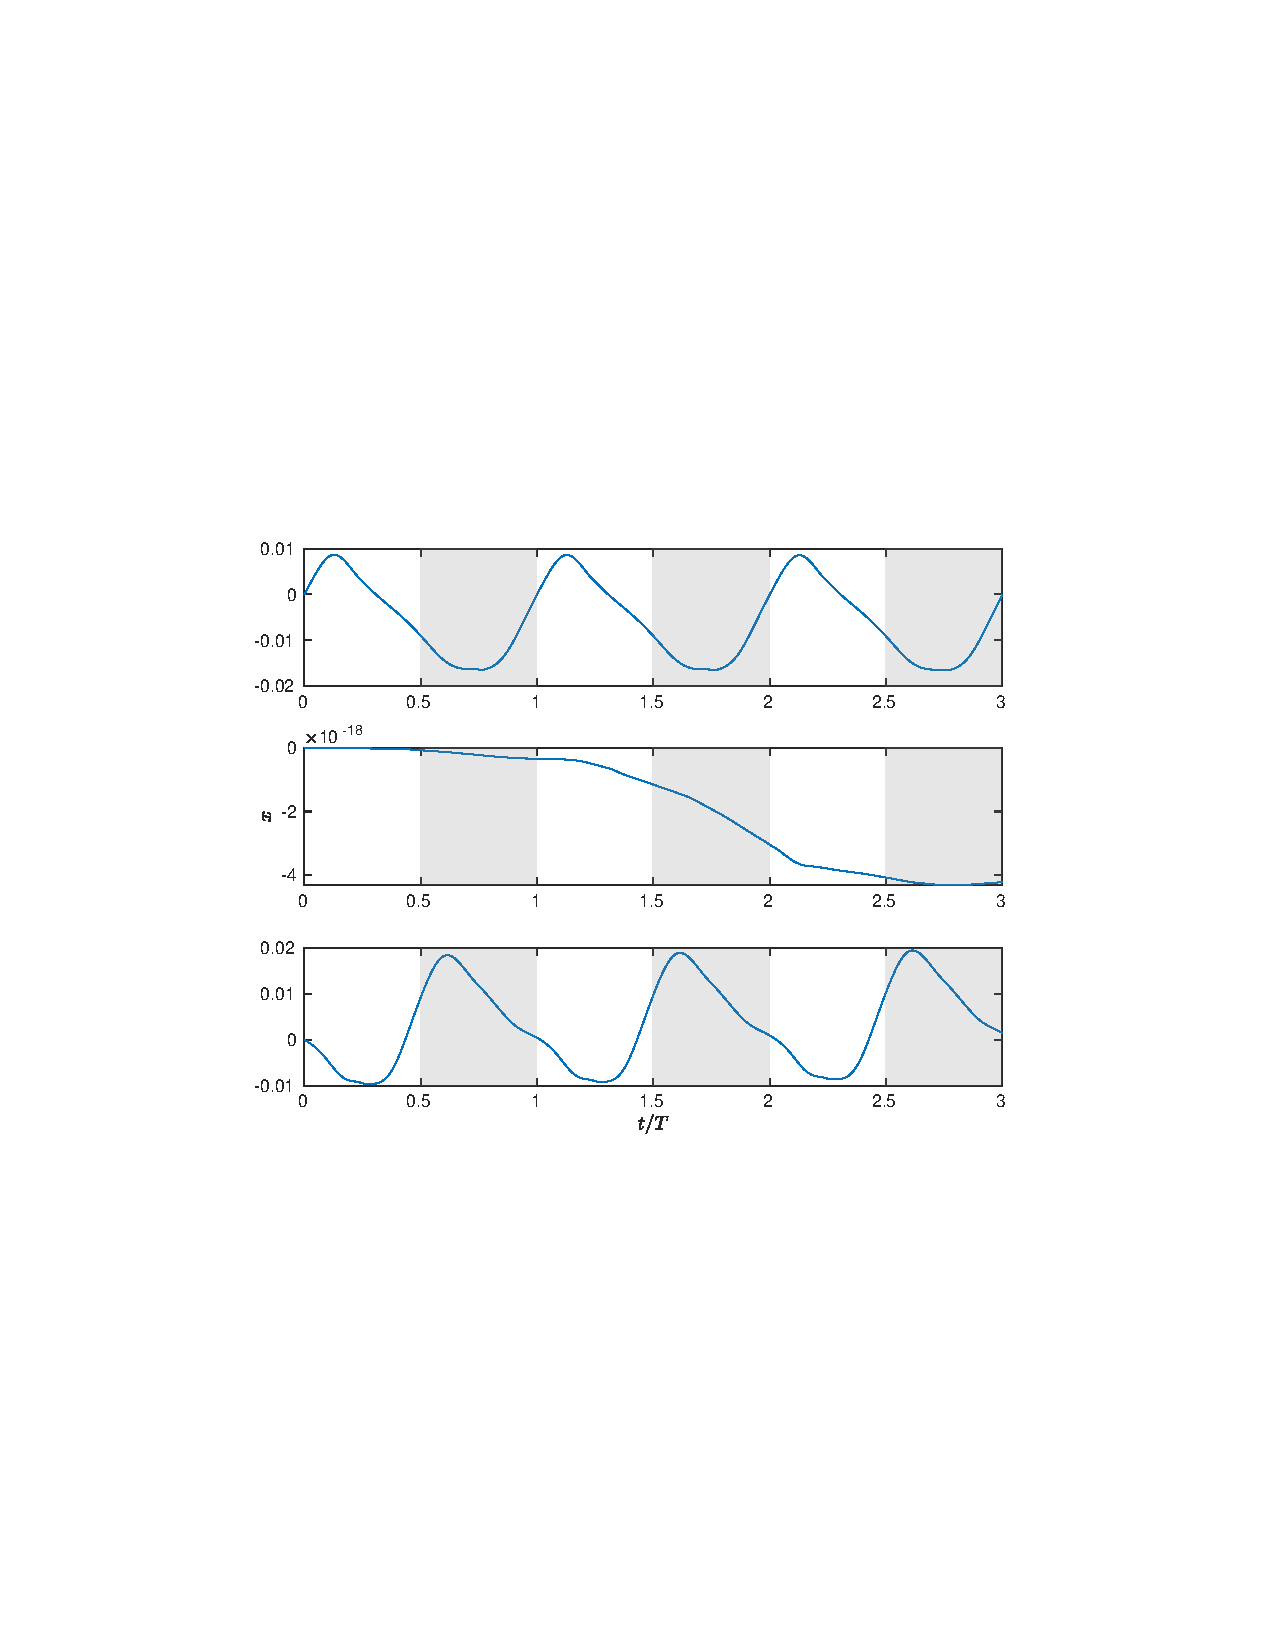
\includegraphics[width=0.75\linewidth]{sim_QS_x_hover_pos.pdf}
%	\caption{Position trajectory}
%\end{figure}
%
%\begin{figure}[h!]
%	\centering
%	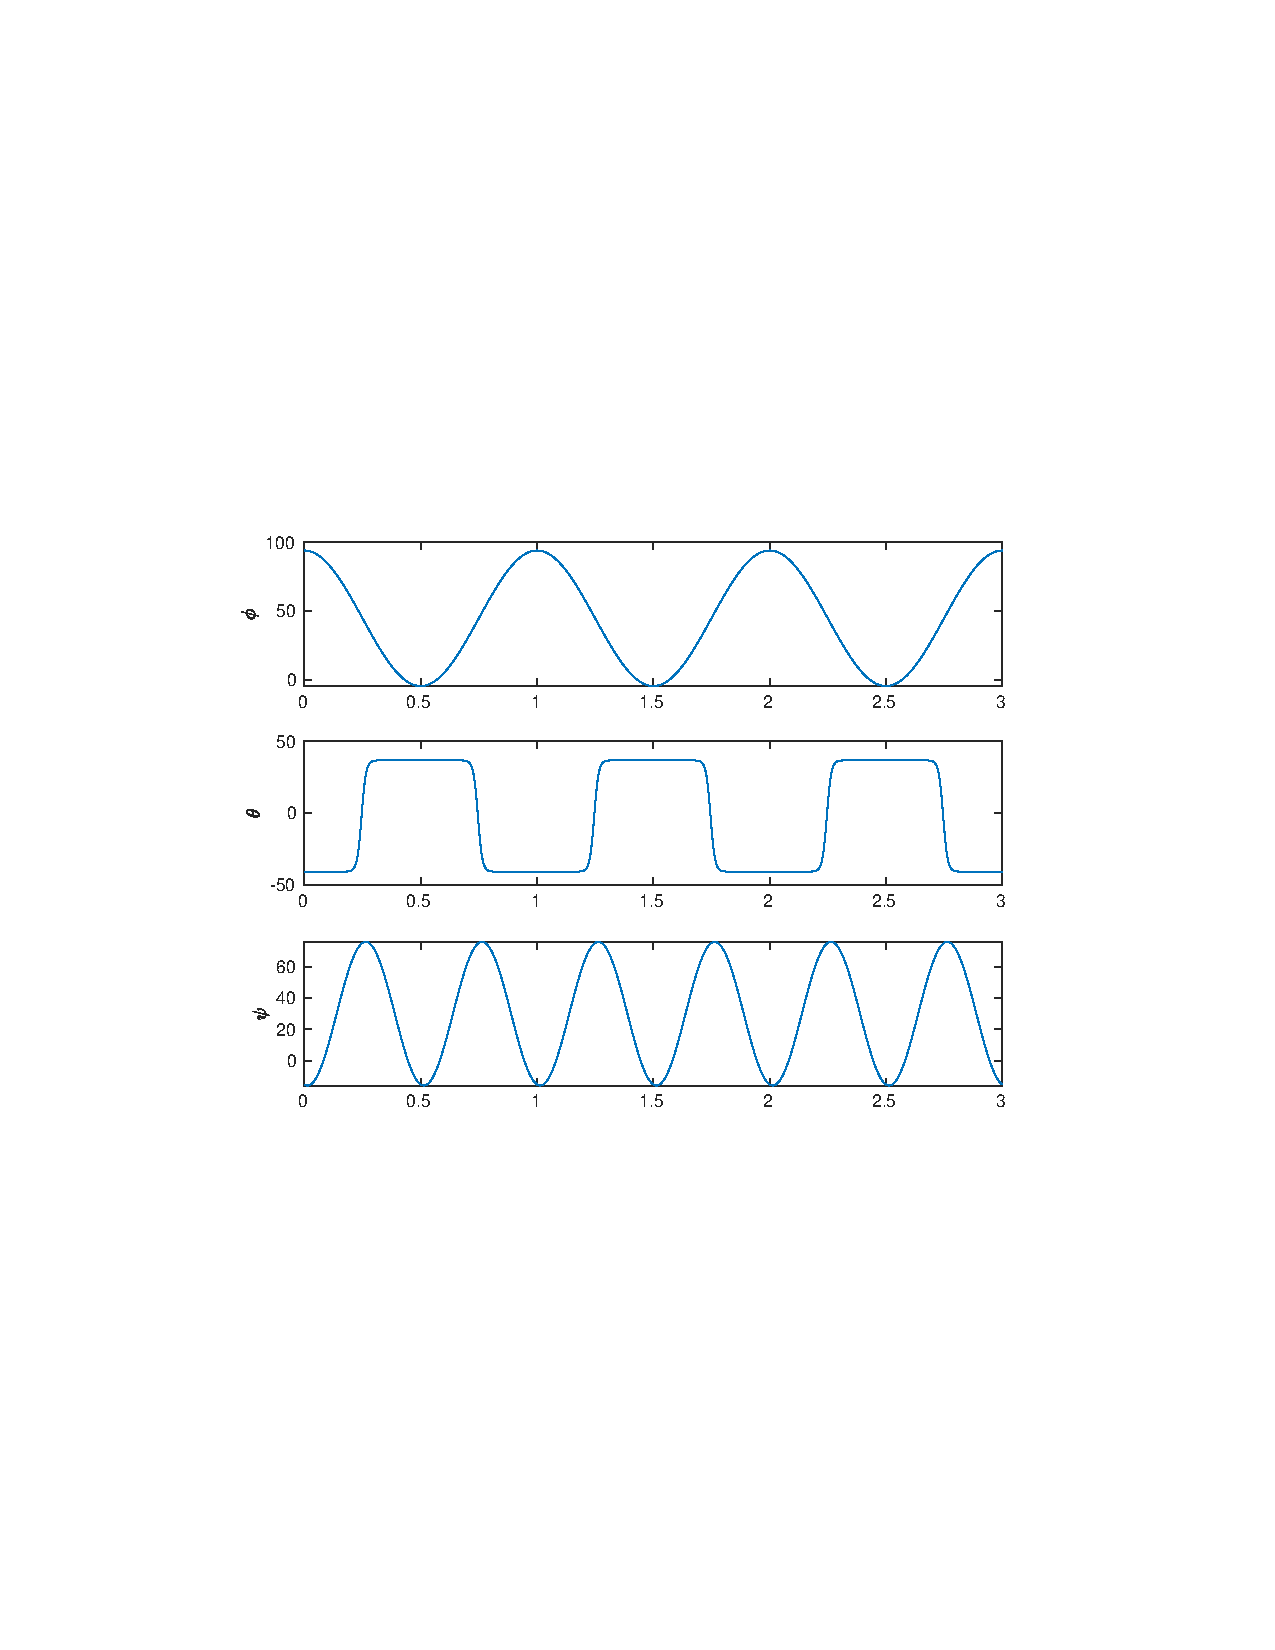
\includegraphics[width=0.75\linewidth]{sim_QS_x_hover_kin.pdf}
%	\caption{Euler angle values}
%\end{figure}

\section{Linearization of dynamics for stability analysis}
We have to find the variational equation with
\[ \delta g = (\delta x, \eta, \eta_R, \eta_L, \eta_A), \delta \xi = (\delta \dot{x}, \delta\Omega, \delta\Omega_R, \delta\Omega_L, \delta\Omega_A) \]
where $ \delta R = R \hat{\eta},\ \dot{\eta} = \delta\Omega - \hat{\Omega} \eta $ for the system:
\begin{gather}
\mathbf{J}_g(\dot \xi) - \ad^*_\xi \cdot \mathbf{J}_g(\xi) + \mathbf{L}_g(\xi) \xi  = \mathbf{f}_a + \mathbf{f}_g + \mathbf{f}_\tau. \label{eqn:EL}
\end{gather}
Hence the linearization of dynamics will look like,
\begin{gather*}
(\delta \mathbf{J}_g) \dot{\xi} + \mathbf{J}_g(\delta \dot{\xi}) - \ad^*_{\delta \xi} \cdot \mathbf{J}_g(\xi) - \ad^*_\xi \cdot \delta \mathbf{J}_g(\xi) - \ad^*_\xi \cdot \mathbf{J}_g(\delta \xi) + \delta (\mathbf{L}_g(\xi)) (\xi) + \mathbf{L}_g(\xi) (\delta \xi) = \delta (\mathbf{f}_a + \mathbf{f}_g + \mathbf{f}_\tau)
%\\
%	\tilde{\mathbf{K}}_g (\delta g) + \mathbf{J}_g(\delta \dot{\xi}) - \tilde{\mathbf{A}}_g(\xi)(\delta \xi) - \ad^*_\xi \cdot \mathbf{K}_g(\xi) (\delta g) - \ad^*_\xi \cdot \mathbf{J}_g(\delta \xi) + (\mathbf{M}_g - \frac{1}{2}\tilde{\mathbf{M}}_g)(\delta g) + (\mathbf{M}_\xi - \frac{1}{2}\tilde{\mathbf{M}}_\xi)(\delta \xi) + \\
%	\mathbf{L}_g(\xi) (\delta \xi)  = (\mathbf{F}_{gravity} + \mathbf{F}_a + \mathbf{F}_\tau) (\delta g)
\end{gather*}
and will have the form,
\begin{align}
	\begin{bmatrix}
	\delta \dot{g} \\ \delta \dot{\xi}
	\end{bmatrix} =
	\begin{bmatrix}
	f_{1,1}(g, \xi) & f_{1,2}(g, \xi) \\ f_{2,1}(g, \xi) & f_{2,2}(g, \xi)
	\end{bmatrix} \begin{bmatrix}
	\delta g \\ \delta \xi
	\end{bmatrix}
\end{align}

\subsection*{Evaluation of all components}
\begin{itemize}
\item  Firstly,
\begin{align*}
\delta \mathbf{J}_i(R,Q_i) \begin{bmatrix}
\ddot{x} \\ \dot{\Omega} \\ \dot{\Omega}_i
\end{bmatrix} = 
\tilde{\mathbf{K}}_i(R, Q_i, \ddot{x}, \dot{\Omega}, \dot{\Omega}_i)
\begin{bmatrix}
\delta x \\ \eta \\ \eta_i
\end{bmatrix}
\end{align*}
where,
\begin{align*}
\tilde{\mathbf{K}}_i(R,Q_i,\ddot{x},\dot{\Omega},\dot{\Omega}_i) = 
\begin{bmatrix}
0 & m_i R ((\hat\mu_i+\widehat{Q_i\nu_i})\dot{\Omega} + Q_i\hat\nu_i\dot{\Omega}_i)^\wedge 
& m_i R( -\hat{\dot{\Omega}} Q_i \hat\nu_i + Q_i \widehat{\hat \nu_i \dot{\Omega}_i}) \\
0 & m_i(\hat\mu_i + \widehat{Q_i\nu_i})\widehat{R^T \ddot{x}}
& m_i\widehat{R^T\ddot{x}}Q_i\hat\nu_i - Q_i (J_iQ_i^T\dot{\Omega})^\wedge + Q_i J_i \widehat{Q_i^T\dot{\Omega}} \\
& & - m_i\hat\mu_i\hat{\dot{\Omega}} Q_i\hat\nu_i - m_i\widehat{\hat\mu_i\dot{\Omega}} Q_i \hat\nu_i \\
& & - Q_i \widehat{J_i\dot{\Omega}_i} + m_i \hat\mu_i Q_i \widehat{\hat\nu_i \dot{\Omega}_i} \\
0 & m_i \hat\nu_i Q_i^T \widehat{R^T\ddot{x}}
& m_i \hat\nu_i (Q_i^T R^T \ddot{x})^\wedge + J_i\widehat{Q_i^T\dot{\Omega}} - m_i\hat\nu_i (Q_i^T\hat\mu_i \dot{\Omega})^\wedge
\end{bmatrix}.
\end{align*}

\begin{align}
\tilde{\mathbf{K}}_g(\dot{\xi}) = \begin{bmatrix}
0 & \tilde{\mathbf{K}}_{R_{12}} + \tilde{\mathbf{K}}_{L_{12}} + \tilde{\mathbf{K}}_{A_{12}} & \tilde{\mathbf{K}}_{R_{13}} & \tilde{\mathbf{K}}_{L_{13}} & \tilde{\mathbf{K}}_{A_{13}}\\
0 & \tilde{\mathbf{K}}_{R_{22}} + \tilde{\mathbf{K}}_{L_{22}} + \tilde{\mathbf{K}}_{A_{22}} & \tilde{\mathbf{K}}_{R_{23}} & \tilde{\mathbf{K}}_{L_{23}} & \tilde{\mathbf{K}}_{A_{23}} \\
0 & \tilde{\mathbf{K}}_{R_{32}} & \tilde{\mathbf{K}}_{R_{33}} & 0 & 0 \\
0 & \tilde{\mathbf{K}}_{L_{32}} & 0 & \tilde{\mathbf{K}}_{L_{33}} & 0 \\
0 & \tilde{\mathbf{K}}_{A_{32}} & 0 & 0 & \tilde{\mathbf{K}}_{A_{33}}
\end{bmatrix}
\end{align}

Thus,
\begin{equation*}
	\delta (\mathbf{J}_g(\dot \xi)) = (\delta \mathbf{J}_g) \dot{\xi} + \mathbf{J}_g \delta \dot{\xi} = \tilde{\mathbf{K}}_g (\dot{\xi}) (\delta g) + \mathbf{J}_g (\delta \dot{\xi})
\end{equation*}

\item  Next,
\begin{align*}
	\delta (\mathrm{ad}^*_\nu)  = 	\mathrm{ad}^*_{\delta \nu} = \mathrm{diag}[0_{3\times 3}, -\delta\hat\Omega, -\delta\hat\Omega_R, -\delta\hat\Omega_L, - \delta\hat\Omega_A] \\
	\implies 
	\delta (\ad^*_\xi \cdot \mathbf{J}_g(\xi)) = \tilde{\mathbf{A}}_g(\xi)(\delta \xi) + \ad^*_\xi \cdot \mathbf{K}_g (\delta g) + \ad^*_\xi \cdot \mathbf{J}_g(\delta \xi)
\end{align*}
where,
\begin{equation} 
\tilde{\mathbf{A}}_g(\xi) = \mathrm{diag}[0_{3\times 3}, {[\mathbf{J}_g(\xi)]_{4:6}}^{\wedge}, {[\mathbf{J}_g(\xi)]_{7:9}}^{\wedge}, {[\mathbf{J}_g(\xi)]_{10:12}}^{\wedge}, {[\mathbf{J}_g(\xi)]_{13:15}}^{\wedge}]
\end{equation}

\item And,
\begin{align*}
\delta \mathbf{K}_i(R,Q_i,\dot{x},\Omega,\Omega_i) \begin{bmatrix}
\dot{x} \\ \Omega \\ \Omega_i
\end{bmatrix}  = \mathbf{M}_{gi}(R,Q_i,\dot{x},\Omega,\Omega_i) \begin{bmatrix}
\delta x \\ \eta \\ \eta_i
\end{bmatrix} + \mathbf{M}_{\xi i}(R,Q_i,\dot{x},\Omega,\Omega_i) \begin{bmatrix}
\delta \dot{x} \\ \delta \Omega \\ \delta \Omega_i
\end{bmatrix}
\end{align*}
where,
\begin{align*}
\mathbf{M}_{gi} &= \begin{bmatrix}
 0 & -m_i R \bigl(((\hat\mu_i+\widehat{Q_i\nu_i})\Omega + Q_i\hat\nu_i\Omega_i)^\wedge \Omega +
 & -m_i R \bigl(\hat{\Omega} (\hat{\Omega} Q_i \hat{\nu}_i - Q_i(\hat{\nu}_i\Omega_i)^\wedge) - \\
 & (-\hat\Omega Q_i \hat\nu_i + Q_i \widehat{\hat \nu_i \Omega_i})\Omega_i\bigr) ^\wedge
 & \hat{\Omega} Q_i (\hat{\nu}_i\Omega_i)^\wedge + Q_i ((\hat{\nu}_i\Omega_i)^\wedge\Omega_i)^\wedge \bigr)\\\\
 0 & - m_i \bigl( (\hat\mu_i + \widehat{Q_i\nu_i}) \hat{\Omega} \widehat{R^T \dot x} + & m_i(\widehat{R^T \dot x} \Omega)^\wedge Q_i \hat{\nu}_i - m_i(\widehat{R^T \dot x}) Q_i (\hat{\nu}_i \Omega_i)^\wedge \\
  & (Q_i \hat{\nu}_i \Omega_i)^\wedge (R^T \dot{x})^\wedge \bigr) & + Q_i ((J_iQ_i^T\Omega)^\wedge \Omega_i)^\wedge + Q_i \hat{\Omega}_i J_i (Q_i^T \Omega)^\wedge - Q_i (J_i \widehat{Q_i^T\Omega}\Omega_i)^\wedge \\
  & & - Q_i J_i \hat{\Omega}_i \widehat{Q_i^T\Omega} + m_i\hat\mu_i\hat\Omega Q_i (\hat\nu_i \Omega_i)^\wedge + m_i\widehat{\hat\mu_i\Omega} Q_i (\hat\nu_i \Omega_i)^\wedge \\
  & & + Q_i (\widehat{J_i\Omega_i} \Omega_i)^\wedge - m_i \hat\mu_i Q_i (\widehat{\hat\nu_i \Omega_i} \Omega_i)^\wedge
  \\\\
 0 & -m_i \hat\nu_i Q_i^T \hat{\Omega} \widehat{R^T\dot x}  & m_i \hat\nu_i (Q_i^T \widehat{R^T\dot x} \Omega)^\wedge -  m_i \hat\nu_i \hat{\Omega}_i (Q_i^T R^T \dot x)^\wedge \\
 & - m_i \hat\nu_i \hat{\Omega}_i Q_i^T (R^T \dot x)^\wedge & - J_i \hat{\Omega}_i \widehat{Q_i^T\Omega} + m_i\hat\nu_i \hat{\Omega}_i (Q_i^T\hat\mu_i \Omega)^\wedge
 \end{bmatrix}
 \\
 \mathbf{M}_{\xi i} &= \begin{bmatrix}
 0 & m_i R (-\hat{\Omega} (\hat{\mu}_i + \widehat{Q_i\nu_i}) + (Q_i \hat{\nu}_i \Omega_i)^\wedge)
 & -m_i R (\hat{\Omega}Q_i\hat\nu_i + Q_i\hat{\Omega}_i\hat{\nu}_i) \\\\
 m_i(\hat\mu_i + \widehat{Q_i\nu_i}) \hat{\Omega}^T R^T &
 Q_i \hat{\Omega}_i (J_iQ_i^T) - Q_i J_i \hat{\Omega}_i Q_i^T & Q_i \hat{\Omega}_i J_i - m_i \hat\mu_i Q_i \hat{\Omega}_i \hat\nu_i  \\
 -m_i(Q_i\hat\nu_i \Omega_i)^\wedge R^T & + m_i\hat\mu_i(Q_i\hat\nu_i\Omega_i)^\wedge + m_i (Q_i\hat\nu_i\Omega_i)^\wedge \hat{\mu}_i & \\\\
 -m_i \hat\nu_i Q_i^T \hat{\Omega} R^T -  m_i \hat\nu_i \hat{\Omega}_i Q_i^T R^T & -J_i \hat{\Omega}_i Q_i^T + m_i\hat\nu_i \hat{\Omega}_i Q_i^T\hat\mu_i & 0
 \end{bmatrix}
\end{align*}
with $ \mathbf{M}_{\xi i} = \mathbf{M}_{\xi i}^T $. Hence,
\begin{equation*}
	\delta (\mathbf{K}_g(\xi)) \xi = \mathbf{M}_g(\xi) (\delta g) + \mathbf{M}_\xi (\xi) (\delta \xi)
\end{equation*}
where,
\begin{align}
{\mathbf{M}_g}(\xi) &= \begin{bmatrix}
0 & {\mathbf{M}_g}_{R_{12}} + {\mathbf{M}_g}_{L_{12}} + {\mathbf{M}_g}_{A_{12}} & {\mathbf{M}_g}_{R_{13}} & {\mathbf{M}_g}_{L_{13}} & {\mathbf{M}_g}_{A_{13}}\\
0 & {\mathbf{M}_g}_{R_{22}} + {\mathbf{M}_g}_{L_{22}} + {\mathbf{M}_g}_{A_{22}} & {\mathbf{M}_g}_{R_{23}} & {\mathbf{M}_g}_{L_{23}} & {\mathbf{M}_g}_{A_{23}} \\
0 & {\mathbf{M}_g}_{R_{32}} & {\mathbf{M}_g}_{R_{33}} & 0 & 0 \\
0 & {\mathbf{M}_g}_{L_{32}} & 0 & {\mathbf{M}_g}_{L_{33}} & 0 \\
0 & {\mathbf{M}_g}_{A_{32}} & 0 & 0 & {\mathbf{M}_g}_{A_{33}}
\end{bmatrix}
\\
{\mathbf{M}_\xi}(\xi) &= \begin{bmatrix}
{\mathbf{M}_\xi}_{R_{11}} + {\mathbf{M}_\xi}_{L_{11}} + {\mathbf{M}_\xi}_{A_{11}}
& {\mathbf{M}_\xi}_{R_{12 }} + {\mathbf{M}_\xi}_{L_{12}} + {\mathbf{M}_\xi}_{A_{12}}
& {\mathbf{M}_\xi}_{R_{13 }}
& {\mathbf{M}_\xi}_{L_{13}} 
& {\mathbf{M}_\xi}_{A_{13}} \\
\cdot & {\mathbf{M}_\xi}_{R_{22}} + {\mathbf{M}_\xi}_{L_{22}} + {\mathbf{M}_\xi}_{A_{22}}
& {\mathbf{M}_\xi}_{R_{23}} 
& {\mathbf{M}_\xi}_{L_{23}} 
& {\mathbf{M}_\xi}_{A_{23}} \\
\cdot & \cdot &  {\mathbf{M}_\xi}_{R_{33}}
& 0 & 0 \\
\cdot & \cdot & 0
& {\mathbf{M}_\xi}_{L_{33}} & 0 \\
\cdot & \cdot & 0 & 0 & {\mathbf{M}_\xi}_{A_{33}}
\end{bmatrix},
\end{align}

\item Similarly,
\begin{align*}
\delta \mathbf{K}_i^T(R,Q_i,\dot{x},\Omega,\Omega_i) \begin{bmatrix}
\dot{x} \\ \Omega \\ \Omega_i
\end{bmatrix}  = \tilde{\mathbf{M}}_{gi}(R,Q_i,\dot{x},\Omega,\Omega_i) \begin{bmatrix}
\delta x \\ \eta \\ \eta_i
\end{bmatrix} + \tilde{\mathbf{M}}_{\xi i}(R,Q_i,\dot{x},\Omega,\Omega_i) \begin{bmatrix}
\delta \dot{x} \\ \delta \Omega \\ \delta \Omega_i
\end{bmatrix}
\end{align*}
where,
\begin{align*}
\tilde{\mathbf{M}}_{gi} = 2 \begin{bmatrix}
0 & 0 & 0 \\\\
\cdot & -m_i ((\hat\mu_i+\widehat{Q_i\nu_i})\Omega + Q_i\hat\nu_i\Omega_i)^\wedge \widehat{R^T\dot{x}} & m_i \widehat{R^T\dot{x}} (\hat{\Omega} Q_i \hat{\nu}_i - Q_i(\hat{\nu}_i\Omega_i)^\wedge) \\\\
\cdot & \cdot & -m_i \bigl( \hat\nu_i (Q_i^T \hat{\Omega} R^T \dot{x})^\wedge + (\hat{\nu}_i\Omega_i)^\wedge (Q_i^T R^T \dot{x})^\wedge \bigr) \\
& & + (J_i Q_i^T \Omega)^\wedge (Q_i^T \Omega)^\wedge -(Q_i^T \Omega)^\wedge J_i (Q_i^T \Omega)^\wedge \\
& & + m_i \hat\nu_i(Q_i^T \hat{\Omega}\hat\mu_i\Omega)^\wedge + \widehat{J_i \Omega_i}\widehat{Q_i^T \Omega} \\
& & + m_i \widehat{\hat{\nu}_i\Omega_i} (Q_i^T \hat\mu_i \Omega)^\wedge \\
\end{bmatrix}
\\
\tilde{\mathbf{M}}_{\xi i} = \begin{bmatrix}
0 & 0 & 0 \\\\
-m_i((\hat\mu_i + \widehat{Q_i\nu_i}) \Omega)^\wedge R^T &  m_i \widehat{R^T \dot{x}} (\hat{\mu}_i + \widehat{Q_i\nu_i})
& m_i\widehat{R^T \dot{x}}Q_i\hat\nu_i\\
-m_i \ (Q_i \hat{\nu}_i \Omega_i)^\wedge R^T  & &
\\\\
-m_i \hat{\nu}_iQ_i^T\hat{\Omega}R^T &  m_i \hat{\nu}_i Q_i^T (R^T \dot{x})^\wedge - \widehat{Q_i^T\Omega}J_iQ_i^T &  m_i (Q_i^T R^T \dot{x})^\wedge \hat\nu_i \\
-m_i \widehat{\hat\nu_i\Omega_i} Q_i^T R^T & + (J_iQ_i^T\Omega)^\wedge Q_i^T -m_i\hat\nu_i Q_i^T \widehat{\hat\mu_i \Omega} & -\widehat{Q_i^T \Omega} J_i \\
& +m_i\hat{\nu}_i Q_i^T \hat{\Omega} \hat\mu_i + \widehat{J_i\Omega_i}Q_i^T + m_i\widehat{\hat\nu_i \Omega_i} Q_i^T\hat\mu_i & - m_i(Q_i^T \hat\mu_i \Omega)^\wedge\hat\nu_i
\end{bmatrix}
\end{align*}
with $ \tilde{\mathbf{M}}_{gi} = \tilde{\mathbf{M}}_{gi}^T $. Hence,
\begin{align*}
\delta(\mathbf{K}^T_g(\xi)) \xi = \tilde{\mathbf{M}}_g(\xi) (\delta g) + \tilde{\mathbf{M}}_\xi(\xi) (\delta \xi)
\end{align*}
where,
\begin{align}
{\tilde{\mathbf{M}}_g}(\xi) &= \begin{bmatrix}
0 & 0 & 0 & 0 & 0\\
\cdot & \tilde{\mathbf{M}}_{gR_{22}} + \tilde{\mathbf{M}}_{gL_{22}} + \tilde{\mathbf{M}}_{gA_{22}} & \tilde{\mathbf{M}}_{gR_{23}} & \tilde{\mathbf{M}}_{gL_{23}} & \tilde{\mathbf{M}}_{gA_{23}} \\
\cdot & \cdot & \tilde{\mathbf{M}}_{gR_{33}} & 0 & 0 \\
\cdot & \cdot & \cdot & \tilde{\mathbf{M}}_{gL_{33}} & 0 \\
\cdot & \cdot & \cdot & \cdot & \tilde{\mathbf{M}}_{gA_{33}}
\end{bmatrix}
\\
{\tilde{\mathbf{M}}_\xi}(\xi) &= \begin{bmatrix}
0 & 0 & 0 & 0 & 0 \\
\tilde{\mathbf{M}}_{\xi R_{21}} + \tilde{\mathbf{M}}_{\xi L_{21}} + \tilde{\mathbf{M}}_{\xi A_{21}} & \tilde{\mathbf{M}}_{\xi R_{22}} + \tilde{\mathbf{M}}_{\xi L_{22}} + \tilde{\mathbf{M}}_{\xi A_{22}}
& \tilde{\mathbf{M}}_{\xi R_{23}} 
& \tilde{\mathbf{M}}_{\xi L_{23}} 
& \tilde{\mathbf{M}}_{\xi A_{23}} \\
\tilde{\mathbf{M}}_{\xi R_{31}} & \tilde{\mathbf{M}}_{\xi R_{32}} &  \tilde{\mathbf{M}}_{\xi R_{33}}
& 0 & 0 \\
\tilde{\mathbf{M}}_{\xi L_{31}} & \tilde{\mathbf{M}}_{\xi L_{32}} & 0
& \tilde{\mathbf{M}}_{\xi L_{33}} & 0 \\
\tilde{\mathbf{M}}_{\xi A_{31}} & \tilde{\mathbf{M}}_{\xi A_{32}} & 0 & 0 & \tilde{\mathbf{M}}_{\xi A_{33}}
\end{bmatrix}
\end{align}

\item On the RHS of dynamics,
\begin{align*}
\delta (\mathbf{f}_{gravity} + \mathbf{f}_a + \mathbf{f}_\tau) = (\mathbf{F}_{gravity} + \mathbf{F}_a + \mathbf{F}_\tau) (\delta g)
\end{align*}
where,
{\small \begin{align}
\mathbf{F}_{gravity} = \begin{bmatrix}
0 & 0 & 0 & 0 & 0 \\
0 & \sum_{i} m_i g (\mu_i + Q_i \nu_i)^\wedge (R^T e_3)^\wedge & m_Rg (R^T e_3)^\wedge Q_R \hat{\nu}_R & m_Lg (R^T e_3)^\wedge Q_L \hat{\nu}_L & m_Ag (R^T e_3)^\wedge Q_A \hat{\nu}_A \\
0 & m_R g \hat\nu_R Q_R^T (R^T e_3)^\wedge & m_R g \hat\nu_R (Q_R^T R^T e_3)^\wedge & 0 & 0\\
0 & m_L g \hat\nu_L Q_L^T (R^T e_3)^\wedge & 0 & m_L g \hat\nu_L (Q_L^T R^T e_3)^\wedge & 0 \\
0 & m_A g \hat\nu_A Q_A^T (R^T e_3)^\wedge & 0 & 0 & m_A g \hat\nu_A (Q_A^T R^T e_3)^\wedge
\end{bmatrix}
\end{align}
\begin{align}
\mathbf{F}_a =  \begin{bmatrix}
0 & \sum_{i} -R(Q_i F_i)^\wedge & -RQ_R\hat{F}_R & -RQ_L\hat{F}_L & -RQ_A\hat{F}_A \\
0 & 0 & -\hat{\mu}_R Q_R \hat{F}_R & -\hat{\mu}_L Q_L \hat{F}_L & -\hat{\mu}_A Q_A \hat{F}_A\\
& & 0_{3 \times 5} & &
\end{bmatrix}
,\mathbf{F}_\tau = \begin{bmatrix}
 & 0_{2\times 5} &  &  \\
 & (Q_R^T \tau_R)^\wedge & 0 & 0 \\
0_{3 \times 2} & 0 & (Q_L^T \tau_L)^\wedge & 0 \\
 &  0 & 0 & (Q_A^T \tau_A)^\wedge
\end{bmatrix}
\end{align}}
\end{itemize}

\textbf{NOTE:} We have not linearized the aerodynamic forces $ F_R, F_L, F_A $ themselves, which if we had done, might help to obtain a better approximation.

\subsection*{Linearized form}
\begin{align*}
	\delta \dot{g} &= \ad^*_{\xi} \cdot \delta g + \mathbf{I}_g(\xi) (\delta \xi) \\
	\delta \dot{\xi} &=  \mathbf{J}_g^{-1} ((-\tilde{\mathbf{K}}_g(\dot{\xi}) + \ad^*_\xi \cdot \mathbf{K}_g(\xi)- \mathbf{M}_g(\xi) + \frac{1}{2}\tilde{\mathbf{M}}_g(\xi) + \mathbf{F}_{gravity} + \mathbf{F}_a + \mathbf{F}_\tau) (\delta g) + \\
	& (\tilde{\mathbf{A}}_g(\xi) + \ad^*_\xi \cdot \mathbf{J}_g - (\mathbf{M}_\xi(\xi) - \frac{1}{2}\tilde{\mathbf{M}}_\xi(\xi)) - \mathbf{L}_g(\xi)) (\delta \xi))
\end{align*}

Denote,
\begin{align*}
	\mathbf{F}_g &:= \mathbf{F}_{gravity} + \mathbf{F}_a + \mathbf{F}_\tau &\mathbf{A}_g(\xi) := \ad^*_\xi\\
	\mathbf{\tilde{L}}_g(\xi) &:= (\mathbf{M}_g - \frac{1}{2}\tilde{\mathbf{M}}_g)(\xi)
	&\mathbf{\tilde{L}}_\xi(\xi) := (\mathbf{M}_\xi - \frac{1}{2}\tilde{\mathbf{M}}_\xi)(\xi)
\end{align*}
\noindent
Thus obtaining,
\begin{align}
	\begin{bmatrix}
	\delta \dot{g} \\\\
	\delta \dot{\xi}
	\end{bmatrix} =
	\begin{bmatrix}
	\mathbf{A}_g(\xi) & \mathbf{I}_g(\xi) \\\\
	\mathbf{J}_g^{-1} (-\tilde{\mathbf{K}}_g(\dot{\xi}) + \mathbf{A}_g(\xi) \mathbf{K}_g(\xi)- \mathbf{\tilde{L}}_g(\xi) + \mathbf{F}_g) &\quad \mathbf{J}_g^{-1} (\tilde{\mathbf{A}}_g(\xi) +  \mathbf{A}_g(\xi) \mathbf{J}_g - \mathbf{\tilde{L}}_\xi(\xi) - \mathbf{L}_g(\xi))
	\end{bmatrix}
	\begin{bmatrix}
	\delta g \\\\
	\delta \xi
	\end{bmatrix}
\end{align}

\section{Linearization of dynamics with prescribed wing kinematics and abdomen/body attitude}

\begin{align*}
m\ddot x + 
\sum_{i\in\{R,L,A\}} \big\{ \mathbf{J}_{i_{12}} \dot\Omega + \mathbf{J}_{i_{13}}\dot\Omega_R 
+ \ \mathbf{K}_{i_{12}}\Omega + \mathbf{K}_{i_{13}}\Omega_i \big\} = R\sum_{i\in\{R,L,A\}} Q_i F_i + mg e_3,\label{eqn:mx_ddot}
\end{align*}
whose perturbation of body position and velocity will yield,
\begin{equation}
	m \frac{d (\delta \dot{x} )}{dt} = R \sum_{i\in\{R,L,A\}} Q_i \delta F_i
\end{equation}
where,
\begin{align*}
	F_R &= L_R + D_R \\
	L_R &= \int_{0}^{l} \frac{1}{2}\rho  C_L(\alpha(r)) \mathrm{sgn} (e_1^T U_R(r) e_3^T U_R(r)) (e_2\times U_R(r))\|U_R(r)\| c(r) dr \\
	D_R &= \int_{0}^{l} - \frac{1}{2}\rho  C_D(\alpha(r)) \|U_R(r)\|U_R(r) c(r) dr \\
	C_L(\alpha) & = 0.225 + 1.58 \sin( (2.13\alpha^\circ - 7.2) \frac{\pi}{180}) \\
	C_D(\alpha) & = 1.92 - 1.55 \cos( (2.04 \alpha^\circ - 9.82 ) \frac{\pi}{180}) \\
	\alpha_R (r) & = \cos^{-1} ( \frac{|e_1^T U_R(r)|}{\|U_R(r)\|} ) \\
	U_R(r) &= (I_{3\times 3}- e_2 e_2^T) Q_R^T( R^T (\dot x-v_{\mathrm{wind}}) + \Omega\times \mu_R ) + r  (Q_R\Omega + \Omega_R )\times e_2
\end{align*}
Hence,
\begin{align*}
	\delta U_R(r) &= (I_{3\times 3}- e_2 e_2^T) Q_R^T R^T \delta\dot x \\
	\delta \alpha_R(r) &= \frac{-1}{\sin(\alpha_R(r))} \mathrm{sgn}(e_1^T U_R(r))\ e_1^T\left(I_{3\times 3} - \frac{U_R(r)U_R^T(r)}{\norm{U_R(r)}^2}\right) \frac{\delta U_R(r)}{\norm{U_R(r)}} \\
	\delta C_L(\alpha(r)) &= 1.58 \cos( (2.13\alpha^\circ - 7.2) \frac{\pi}{180}) \times 2.13\ \delta\alpha_R(r) \\
	\delta C_D(\alpha(r)) &= 1.55 \sin( (2.04 \alpha^\circ - 9.82 ) \frac{\pi}{180}) \times 2.04\ \delta\alpha_R(r) \\
%	\delta L_R &= \delta \int_{0}^{l} \frac{1}{2}\rho  C_L(\alpha(r)) \mathrm{sgn} (e_1^T U_R(r) e_3^T U_R(r)) (e_2\times U_R(r))\|U_R(r)\| c(r) dr 
\end{align*}

Substituting back these values obtain $ \delta F_R, \delta F_L $. Using these expressions, the perturbation plot is shown in \cref{fig:pos_vel_pert} and it is observed that the disturbance in velocity is damped.

\begin{figure}[h]
	\centering
	\includegraphics[width=0.6\linewidth]{sim_QS_x_hover_stability.eps}
	\caption{Position and velocity perturbations}
	\label{fig:pos_vel_pert}
\end{figure}

Comparing the various kinds of flying insects, one might expect the nature of perturbation to change with flapping frequency. We have a comparison plot in \cref{fig:vel_damping}.

\begin{figure}[H]
	\centering
	\includegraphics[width=0.9\linewidth]{convergence_rate.pdf}
	\caption{Rate of convergence of perturbation for different insects}
	\label{fig:vel_damping}
\end{figure}

Using floquet theory, since the values of all the characteristic multipliers, $ \norm{\rho_i} \le 1 $ (\cref{fig:char_multipliers}), the perturbed system is stable.
\begin{figure}[H]
	\centering
	\includegraphics[width=0.4\linewidth]{char_multipliers.eps}
	\caption{Complex value plot of the characteristic multipliers of  perturbed system}
	\label{fig:char_multipliers}
\end{figure}

\end{document}